
\includegraphics[height=1.25cm]{images/pictograms/benchmark}

\includegraphics[height=1.25cm]{images/pictograms/FEM}

\includegraphics[height=1.25cm]{images/pictograms/3d}

%%%%%%%%%%%%%%%%%%%%%%%%%%%%%%%%%%%%%%%%%%%%%%%%%%%%%%%%%%%%%%%%%%%%%%%%%%%%%%%%%%%%%%%%%%%%%%%%%%%

\lstinputlisting[language=bash,basicstyle=\small]{python_codes/fieldstone_91/keywords.ascii}

\begin{center}
Code at \url{https://github.com/cedrict/fieldstone/tree/master/python_codes/fieldstone_91}
\end{center}

\par\noindent\rule{\textwidth}{0.4pt}

%%%%%%%%%%%%%%%%%%%%%%%%%%%%%%%%%%%%%%%%%%%%%%%%%%%%%%%%%%%%%%%%%%%%%%%%%%%%%%%%%%%%%%%%%%%%%%%%%%%%


This \stone carries out the Stokes sphere benchmark of 
Section~\ref{MMM-ss:stokes_sphere3D} although 
it uses an axisymmetric formulation, so that the sphere is actually falling inside 
a vertical cylinder. As a consequence, the boundary conditions are: 
free slip on the left (the axis of symmetry), top and bottom, and no slip on the right (the
wall of the cylinder). The default domain size is $L_r=0.5$ and $L_z=1$.

Having established the weak form of the Stokes equations and discretised them in 
Section~\ref{MMM-ss:cyl_axi}, transforming a 2D plane-strain code into an axisymmetric 
one is rather straightforward. In a nutshell, 
\begin{itemize}
\item $x$ stands for $r$
\item $\upnu_r$ is $u$, $\upnu_z$ is $w$
\item the matrix ${\bm B}$ goes from 
$3 \times m_v\cdot ndofV$ to $4 \times m_v\cdot ndofV$. 
\item the matrix ${\bm N}$ goes from $3 \times m_p\cdot ndofP$ to $4 \times m_p\cdot ndofP$. 
\item the matrix ${\bm C}$ goes from $3 \times 3$ to $4 \times 4$.
\item integrals must be multiplied by $2 \pi$ and also contain an additional $r$ term
which translates into $x_q$ in the code. 
\end{itemize}

The Stokes sphere velocity is given by
\[
\upnu_{Stokes} = \frac{2}{9} \frac{\delta \rho}{\eta_f} R_s^2 g
\]
which yields $\upnu_S\simeq 3.387 \cdot 10^{-5}$. However, 
this is for a sphere in an infinite domain. When placed in a 
cylinder, the influence of the walls will slow the sphere down. 
Two corrections have been proposed be Habermann and by Faxen.

We start by writing the drag force
\[
F_H = 6 \pi \eta_f R \upnu_{sphere}\;  \gamma\left(\frac{r}{R}\right) 
\]
In the case of the Stokes sphere in an infinite medium then $\gamma =1$ and equating
$F_H$ with the buoyancy force $4/3 \pi R^3 \delta\rho g$ yields the above velocity.
Habermann gives a coefficient $\gamma$ such that 
\[
\gamma\left(\frac{r}{R}\right)  = 
\frac{1-0.75857 \left(\frac{r}{R}\right)^5}{1+f_H\left(\frac{r}{R}\right)}
\]
with 
\[
f_H\left(\frac{r}{R}\right) 
= -2.1050\left(\frac{r}{R}\right)+ 2.0865\left(\frac{r}{R}\right)^3
- 1.7068\left(\frac{r}{R}\right)^5 + 0.72603\left(\frac{r}{R}\right)^6 
\]
Faxen gives a coefficient $\gamma$ such that 
\[
\gamma\left(\frac{r}{R}\right) = \frac{1}{1 + f_F\left(\frac{r}{R}\right)} 
\]
with 
\[
f_F\left(\frac{r}{R}\right) 
= -2.10444 \left(\frac{r}{R}\right) 
+ 2.08877\left(\frac{r}{R}\right)^3 
- 0.94813\left(\frac{r}{R}\right)^5 
- 1.372\left(\frac{r}{R}\right)^6 
+ 3.87\left(\frac{r}{R}\right)^8 
- 4.19\left(\frac{r}{R}\right)^{10}
\]
In all three cases we have 
\[
\upnu_{sphere} = \frac{2}{9} \frac{\delta \rho}{\eta_f} R_s^2 g \frac{1}{\gamma(\frac{r}{R})}
\]
Note that the Habermann \& Faxen expressions are copy-pasted from the GALE manual and 
are extremely comparable in value. I did not verify these yet. 
Please check Lindgren (1999) \cite{lind99} to do so. They are 
about half the value of the Stokes velocity
in this case. The three velocity values are computed directly in the 
code and exported alongside
the measured velocity.

We see that increasing the height of the cylinder does not substantially 
alter the results, and that 
the velocity in the middle of the sphere seems to converge to the expected ones:
\begin{center}
\includegraphics[width=5cm]{python_codes/fieldstone_91/results/vc.pdf}
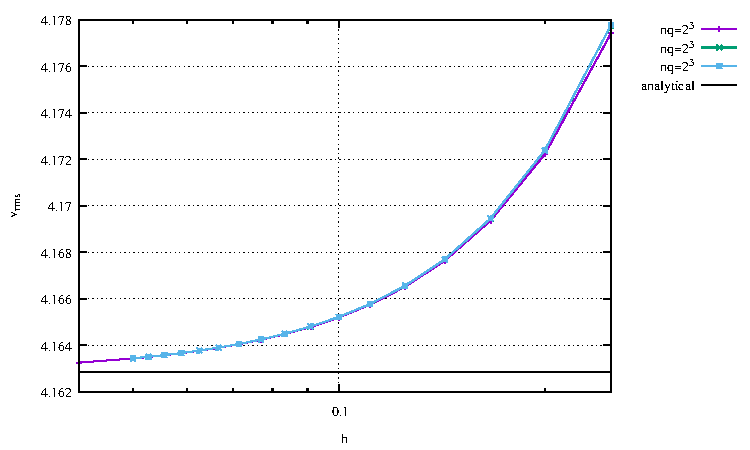
\includegraphics[width=5cm]{python_codes/fieldstone_91/results/vrms.pdf}
\includegraphics[width=5cm]{python_codes/fieldstone_91/results/mass.pdf}\\
{\captionfont up to $256 \times 512$ elements.}
\end{center}


\begin{center}
\includegraphics[width=4cm]{python_codes/fieldstone_91/results/ps/vel}
\includegraphics[width=4cm]{python_codes/fieldstone_91/results/ps/press}
\includegraphics[width=4cm]{python_codes/fieldstone_91/results/ps/exx}
\includegraphics[width=4cm]{python_codes/fieldstone_91/results/ps/exy}\\
\includegraphics[width=4cm]{python_codes/fieldstone_91/results/axi/vel}
\includegraphics[width=4cm]{python_codes/fieldstone_91/results/axi/press}
\includegraphics[width=4cm]{python_codes/fieldstone_91/results/axi/exx}
\includegraphics[width=4cm]{python_codes/fieldstone_91/results/axi/exy}\\
{\captionfont Top row: plane strain; Bottom row: axisymmetric. Resolution $50\times 100$.}
\end{center}


